\documentclass[12pt]{article}

\setlength{\topmargin}{-.75in} \addtolength{\textheight}{2.00in}
\setlength{\oddsidemargin}{.00in} \addtolength{\textwidth}{.75in}

\usepackage{amsmath,color,graphicx,array,multirow,rotating, enumerate}
\usepackage{type1cm}
\usepackage{eso-pic}
\usepackage[hmargin=2cm,vmargin=1.3cm]{geometry}
\usepackage{mathabx}
\usepackage[rflt]{/Users/jgates/desktop/latex/floatflt}
\usepackage[table]{xcolor}
\nofiles

\def\Tab#1{\tabular[t]{>{\rule[-1ex]{0pt}{3ex}}c}#1\endtabular}
\newcolumntype{C}{@{}c@{}}

\pagestyle{empty}
\newcounter{ProbNum}
\setlength{\parindent}{0in}

% Watermark: graph paper
\newcommand\BackgroundPic{
\put(0,0){
\parbox[b][\paperheight]{\paperwidth}{%
\vfill
\centering

\includegraphics[width=\paperwidth,height=\paperheight,keepaspectratio]{/Users/jgates/desktop/latex/pics/plain.pdf}%
\vfill
}}}

%Diagram box command [v space][content]
\newcommand{\diagrambox}[2][40 mm]{
\framebox{\parbox{175 mm}{#2 \hfill \\ \vspace{#1}}}

\bigskip
}

% MakeList: [example number] [content]
\newcommand{\MakeList}[2]{
\begin{enumerate}[#1] \itemsep1pt \parskip0pt \parsep0pt  

#2
\end{enumerate}
}

\begin{document}



% Name section
\noindent {\sc {\bf {\Large Recitation Problems }} \hfill
}

\noindent {\sc Honors Physics }\hfill {\large 6/07}
\bigskip

% Questions section
% Number 490
% Recitation
% Recitation Packet Cover 
% JG/KO


{\bf {\Huge Honors Physics Fall Term \\ Recitation Problems}}

\bigskip
{\large Tips about this packet:
\begin{itemize} \itemsep1pt \parskip0pt \parsep0pt 
\renewcommand{\labelitemi}{$\rightarrow$}
\item Everyone should do every problem!
\item Put your work on the left-hand page. Use the right-right page for notes during presentations
\item Each person will present one problem to the class (approximately 10 minutes) near the end of the term
\item Choosing a problem that looks hard/scary/unfamiliar can allow you to become an expert in that, turning a weakness into a strength
\item The presentations will not be graded, but will be really helpful in preparing for the exam
\item Checking your solutions/answers with me before presentation day is a great idea (you'll only get 10 minutes to present in class, no matter what!)
\item There's no guarantee offered that this covers every piece of every standard from the term, but it's a great place to practice for the exam.
\end{itemize}}

\newpage

% Number 600
% CAPMA CAPMG Algebra Units 
% Overtaking - CAPM and CVPM
% JG

% Watermark
\AddToShipoutPicture*{\BackgroundPic}

\addtocounter {ProbNum} {1}

%\begin{floatingfigure}[r]{.2\textwidth}
%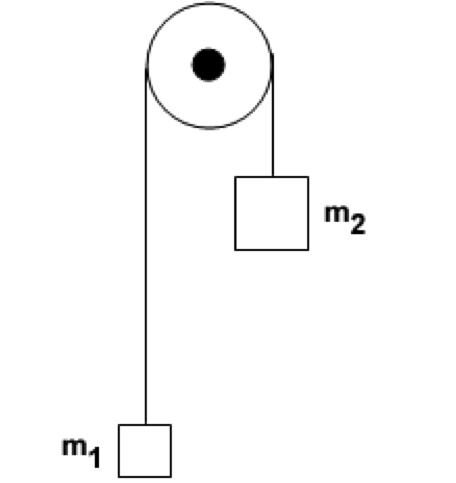
\includegraphics[scale=.8]{/Users/jgates/desktop/latex/pics/Atwood3}
%\end{floatingfigure}
 
{\bf \Large{\arabic{ProbNum}}} A police car is driving towards a parked pair of criminals eating Zagnuts after pulling off a heist. The police car is moving ${40~\tfrac{m}{s}}$ and is initially .4 km away from the criminals. The criminals are going to drive away from the police car in an attempt to escape.  Assume that the crimemobile moves with a constant acceleration of ${1.8~\tfrac{m}{s^2}}$. 

\bigskip
Where will the police catch them?

\vfill

Draw a velocity graph for the criminals.  Use it to determine how far down they road they are when the police car passes their starting point.
\vfill

%\hfill 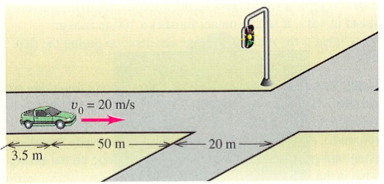
\includegraphics[scale=.85]{/Users/jgates/desktop/latex/pics/redlight.png}
\newpage
% Number 491
% Recitation
% Recitation Packet Separator Sheet 
% JG/KO

% Watermark
\AddToShipoutPicture*{\BackgroundPic}


\bigskip
{\large Presented by: }\underline{\hspace{5cm}}




\vfill
\newpage

% Number 500
% CAPMA CVPMA 
% Stoplight stopping
% KO

% Watermark
\AddToShipoutPicture*{\BackgroundPic}

\addtocounter {ProbNum} {1}

%\begin{floatingfigure}[r]{.33\textwidth}
%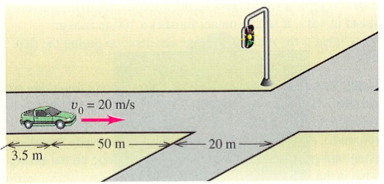
\includegraphics[scale=.6]{/Users/jgates/desktop/latex/pics/redlight}
%\end{floatingfigure}
 
{\bf \Large{\arabic{ProbNum}}} A car 3.5 m in length and traveling at a constant speed of ${20~\tfrac{m}{s}}$ is approaching an intersection. The width of the intersection is 20 m. The light turns yellow when the front of the car is 50 m from the beginning of the intersection. If the driver steps on the brake, the car will slow at a rate of ${4.2~\tfrac{m}{s}}$ per second. If the driver instead steps on the gas pedal, the car will accelerate at ${1.5~\tfrac{m}{s^2}}$. The light will be yellow for 3 seconds. Ignore the reaction time of the driver. 

\bigskip
To avoid being in the intersection while the light is red, should the driver hit the brake pedal or the gas pedal? Justify your answer with some pretty physics.

\hfill 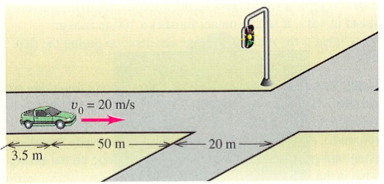
\includegraphics[scale=.85]{/Users/jgates/desktop/latex/pics/redlight.png}


\vfill
\newpage

% Number 491
% Recitation
% Recitation Packet Separator Sheet 
% JG/KO

% Watermark
\AddToShipoutPicture*{\BackgroundPic}


\bigskip
{\large Presented by: }\underline{\hspace{5cm}}




\vfill
\newpage

% Number 540
% UFPM Vectors Algebra Units CAPMA CVPMA
% Wagon rolling down hill
% KO/JG

% Watermark
\AddToShipoutPicture*{\BackgroundPic}

\addtocounter {ProbNum} {1}

%\begin{floatingfigure}[r]{.45\textwidth}
%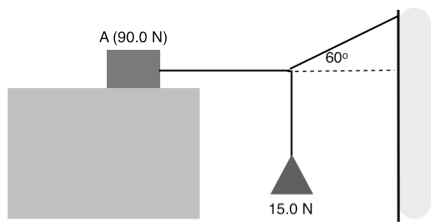
\includegraphics[scale=.6]{/Users/jgates/desktop/latex/pics/static1}
%\end{floatingfigure}
 
{\bf \Large{\arabic{ProbNum}}} A wagon with two boxes of gold (total mass 300 kg) is cut loose from the horses by an outlaw when the wagon is at rest 50 m up a 6 degree slope. The outlaw plans to have the wagon roll down the slope and across the level ground, and then fall into a canyon where his confederates wait. 

\bigskip
Find the speed of the wagon when it reaches the flat ground. Note that it starts from rest at the top of the incline and that the wagon rolls with negligible friction.

\vfill

\vfill
If another bandit standing at the end of the slope requires twenty seconds to grab the gold, how far must the edge of the cliff be from the end of the slope, in order to make this double-heist successful?

%\hfill 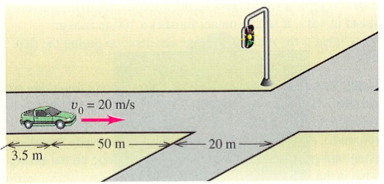
\includegraphics[scale=.85]{/Users/jgates/desktop/latex/pics/redlight.png}


\vfill
\newpage

% Number 491
% Recitation
% Recitation Packet Separator Sheet 
% JG/KO

% Watermark
\AddToShipoutPicture*{\BackgroundPic}


\bigskip
{\large Presented by: }\underline{\hspace{5cm}}




\vfill
\newpage

% Number 530
% UFPM SFriction KFriction Algebra Units CAPMA
% Sliding crate on truck bed - friction
% KO

% Watermark
\AddToShipoutPicture*{\BackgroundPic}

\addtocounter {ProbNum} {1}

%\begin{floatingfigure}[r]{.45\textwidth}
%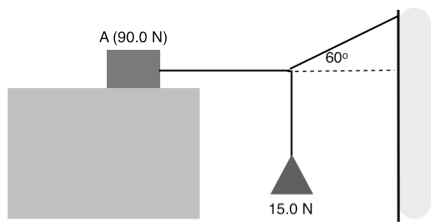
\includegraphics[scale=.6]{/Users/jgates/desktop/latex/pics/static1}
%\end{floatingfigure}
 
{\bf \Large{\arabic{ProbNum}}} A 20 kg box rests on the flat floor of a truck. The coefficients of friction between the box and floor are ${\mu_s=.15}$ and ${\mu_k=.1}$. The truck stops gently at a stop sign and then starts to move with a constant acceleration. The box is 2.2 m from the rear of the truck when the truck starts.

\bigskip
What is the maximum possible acceleration that the truck may have if the box is not to slide?

\vfill
Suppose that the acceleration of the truck is instead ${2.1~\tfrac{m}{s^2}}$. How much time elapses before the box falls off the rear of the truck? 

\vfill
How far does the truck travel in this time?

%\hfill 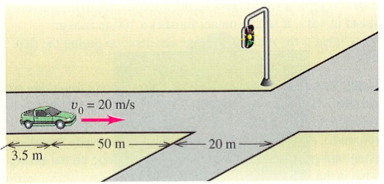
\includegraphics[scale=.85]{/Users/jgates/desktop/latex/pics/redlight.png}


\vfill
\newpage

% Number 491
% Recitation
% Recitation Packet Separator Sheet 
% JG/KO

% Watermark
\AddToShipoutPicture*{\BackgroundPic}


\bigskip
{\large Presented by: }\underline{\hspace{5cm}}




\vfill
\newpage

% Number 590
% UFPM  Inclines CAPMA CAPMG Algebra Units 
% Cart sliding up incline
% JG

% Watermark
\AddToShipoutPicture*{\BackgroundPic}

\addtocounter {ProbNum} {1}

%\begin{floatingfigure}[r]{.2\textwidth}
%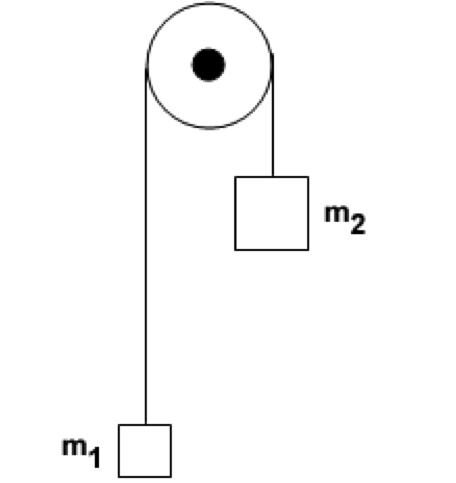
\includegraphics[scale=.8]{/Users/jgates/desktop/latex/pics/Atwood3}
%\end{floatingfigure}
 
{\bf \Large{\arabic{ProbNum}}} A glider is given a quick push to start it moving up a ${7^{\circ}}$ inlined air track. The glider travels to a maximum distance of 112 cm up the track.

\bigskip
Determine the initial speed of the glider.
 
\vfill
\vfill

Draw a velocity graph for the glider; use the graph to determine how long the glider takes to get to that 112 cm point.
\vfill

Use your velocity graph to determine where the glider will be 2 seconds after it was launched.
\vspace{30 mm}
%\hfill 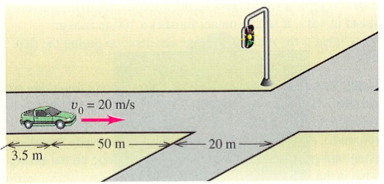
\includegraphics[scale=.85]{/Users/jgates/desktop/latex/pics/redlight.png}
\newpage
% Number 491
% Recitation
% Recitation Packet Separator Sheet 
% JG/KO

% Watermark
\AddToShipoutPicture*{\BackgroundPic}


\bigskip
{\large Presented by: }\underline{\hspace{5cm}}




\vfill
\newpage

% Number 580
% UFPM Tension Algebra Prefixes Units 
% Atwood - bounce height?
% JG

% Watermark
\AddToShipoutPicture*{\BackgroundPic}

\addtocounter {ProbNum} {1}

\begin{floatingfigure}[r]{.2\textwidth}
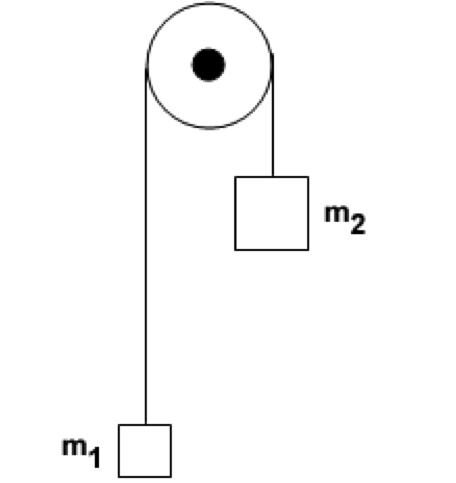
\includegraphics[scale=.8]{/Users/jgates/desktop/latex/pics/Atwood3}
\end{floatingfigure}
 
{\bf \Large{\arabic{ProbNum}}} An Atwood machine is constructed from a 3 kg mass and a 1 kg mass.  The 3 kg mass is released from rest 180 cm off of the floor, while the 1 kg mass is 40 cm above the floor.

\bigskip
Determine the speed of the 3 kg mass as it hits the floor.
\paragraph{}
\noindent
\vfill

After the 3 kg mass hits the floor, the 1 kg mass will continue to move upwards for a short time.  Determine how high above the floor the 1 kg mass will rise.
\vfill

Draw quantitatively correct acceleration and velocity graphs for the 1 kg mass.
\vfill
%\hfill 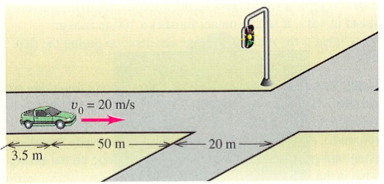
\includegraphics[scale=.85]{/Users/jgates/desktop/latex/pics/redlight.png}
\newpage
% Number 491
% Recitation
% Recitation Packet Separator Sheet 
% JG/KO

% Watermark
\AddToShipoutPicture*{\BackgroundPic}


\bigskip
{\large Presented by: }\underline{\hspace{5cm}}




\vfill
\newpage

% Number 571
% UFPM Tension Algebra Units 
% Elevator with counterweight; graph a vs. F
% JG

% Watermark
\AddToShipoutPicture*{\BackgroundPic}

\addtocounter {ProbNum} {1}

\begin{floatingfigure}[r]{.2\textwidth}
\includegraphics[scale=.8]{/Users/jgates/desktop/latex/pics/elevatorcw}
\end{floatingfigure}
 
{\bf \Large{\arabic{ProbNum}}} An elevator (1500 kg mass, with passengers) is attached to a 1000 kg counterweight by a cable that is wrapped over a pulley, as shown.  It is also attached (by a second cable) to a motor.  The elevator is moving down at a constant speed of 5 meters per second.

\bigskip
Determine the force that the motor must apply to the second cable.
\paragraph{}
\noindent
\vfill
\vfill

Determine the force that the motor must exert to lower the elevator with a constant downward acceleration of ${1~\tfrac{m}{s^2}}$.

\vfill
\vfill
Determine the force that the motor must exert to lower the elevator with a constant upward acceleration of  ${1~\tfrac{m}{s^2}}$.

\vfill
%\hfill 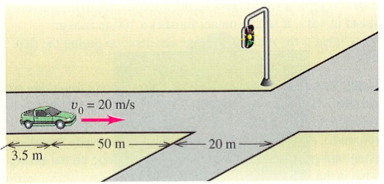
\includegraphics[scale=.85]{/Users/jgates/desktop/latex/pics/redlight.png}
Draw a graph of the acceleration of the elevator as a function of the force exerted by the motor.  Fill in important numbers on each axis.

\vfill
\vfill
\newpage
% Number 491
% Recitation
% Recitation Packet Separator Sheet 
% JG/KO

% Watermark
\AddToShipoutPicture*{\BackgroundPic}


\bigskip
{\large Presented by: }\underline{\hspace{5cm}}




\vfill
\newpage

% Number 550
% UFPM SFriction Algebra Units CAPMA KFriction
% Block held up to vertical cart by acceleration/friction
% KO/JG

% Watermark
\AddToShipoutPicture*{\BackgroundPic}

\addtocounter {ProbNum} {1}

\begin{floatingfigure}[r]{.2\textwidth}
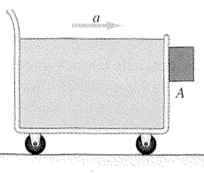
\includegraphics[scale=.6]{/Users/jgates/desktop/latex/pics/cartstatic}
\end{floatingfigure}
 
{\bf \Large{\arabic{ProbNum}}} The cart accelerates to the right, keeping block A from sliding down. The coefficient of static friction between the block and the cart is .8, and the coefficient of kinetic friction is .5. The block is 1.2 meters above the ground.

\bigskip
What minimum acceleration must the cart have in order that block A does not fall? 

\vfill
If the acceleration of the cart were only half that value, how long would it take for the block to hit the ground?
%\hfill 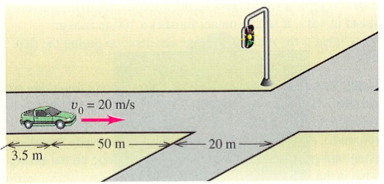
\includegraphics[scale=.85]{/Users/jgates/desktop/latex/pics/redlight.png}

\vfill
\vfill
\newpage

% Number 491
% Recitation
% Recitation Packet Separator Sheet 
% JG/KO

% Watermark
\AddToShipoutPicture*{\BackgroundPic}


\bigskip
{\large Presented by: }\underline{\hspace{5cm}}




\vfill
\newpage

% Number 610
% UFPM SFriction Friction Tension Vectors Algebra Units 
% Pulling box at angle - min angle?
% JG

% Watermark
\AddToShipoutPicture*{\BackgroundPic}

\addtocounter {ProbNum} {1}

\begin{floatingfigure}[r]{.35\textwidth}
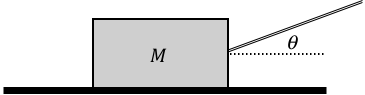
\includegraphics[scale=.6]{/Users/jgates/desktop/latex/pics/pullingbox1}
\end{floatingfigure}
 
{\bf \Large{\arabic{ProbNum}}} A 10 kg box is pulled across the floor by a rope inclined ${21^{\circ}}$ from the horizontal. The coefficient of static friction between the floor and the box is .7 and the coefficient of kinetic friction is .4. 

\bigskip
How hard will the rope need to be pulled in order to set the box in motion?
\paragraph{}
\noindent
\vfill

If the angle is changed, the necessary force to make the box slide changes. Determine the angle at which the tension required to move the box is at a minimum.  You may need to get creative to find that minimum point!
\vfill

%\hfill 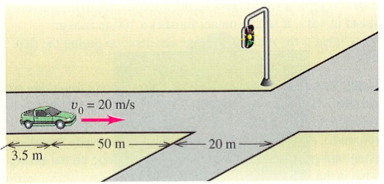
\includegraphics[scale=.85]{/Users/jgates/desktop/latex/pics/redlight.png}
\newpage
% Number 491
% Recitation
% Recitation Packet Separator Sheet 
% JG/KO

% Watermark
\AddToShipoutPicture*{\BackgroundPic}


\bigskip
{\large Presented by: }\underline{\hspace{5cm}}




\vfill
\newpage

% Number 620
% UFPM CAPMG Algebra Units
% Graphs: F to a to delta v, varying F
% JG

% Watermark
\AddToShipoutPicture*{\BackgroundPic}

\addtocounter {ProbNum} {1}

\begin{floatingfigure}[r]{.54\textwidth}
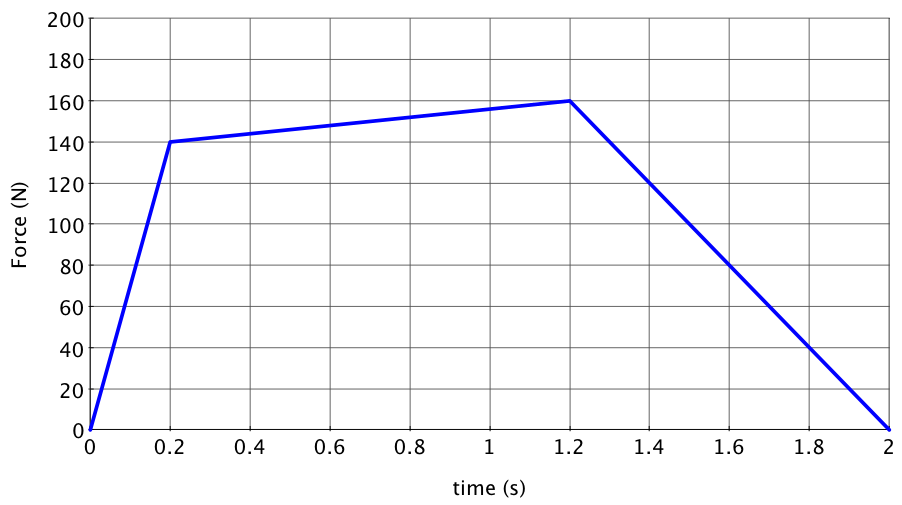
\includegraphics[scale=.7]{/Users/jgates/desktop/latex/pics/Fvst1}
\end{floatingfigure}
 
{\bf \Large{\arabic{ProbNum}}} A 50 kg peewee football player runs into a stationary 40 kg player at an initial speed of 4 meters per second. The magnitude of the force exerted by the football players on each other is shown as a function of time. 

\bigskip
Draw quantitatively accurate acceleration graphs for each player.
\paragraph{}
\noindent
\vfill
Use your acceleration graphs to determine the players' final velocities.
\vfill

Draw a motion diagram showing the players' motions before and after the collision.
\vspace{20mm}

%\hfill 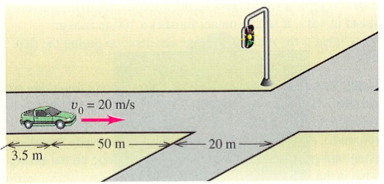
\includegraphics[scale=.85]{/Users/jgates/desktop/latex/pics/redlight.png}
\newpage
% Number 491
% Recitation
% Recitation Packet Separator Sheet 
% JG/KO

% Watermark
\AddToShipoutPicture*{\BackgroundPic}


\bigskip
{\large Presented by: }\underline{\hspace{5cm}}




\vfill
\newpage

% Number 520
% BFPM SFriction Vectors Algebra Units Tension
% Balanced forces - multiple ropes, static friction
% KO

% Watermark
\AddToShipoutPicture*{\BackgroundPic}

\addtocounter {ProbNum} {1}

\begin{floatingfigure}[r]{.45\textwidth}
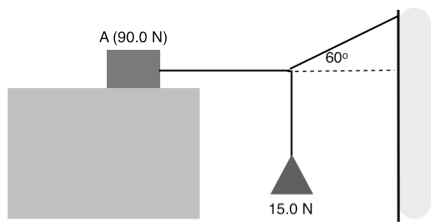
\includegraphics[scale=.6]{/Users/jgates/desktop/latex/pics/static1}
\end{floatingfigure}
 
{\bf \Large{\arabic{ProbNum}}} In the diagram, there is a block (Block A) with weight 90.0 N resting on the table. The coefficient of static friction between the block and the surface on which it rests is 0.30. Block A is connected to a hanging mass with weight 15.0 N. The hanging mass is also connected to the wall, with the angle of the connecting string being 60 degrees.

\bigskip
Determine the force of friction that must be acting on Block A if the entire system is at rest.
\paragraph{}
\noindent
\vfill
Determine the maximum weight that the hanging mass may have, if all other conditions stay the same.

%\hfill 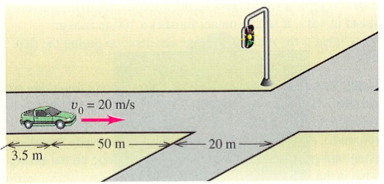
\includegraphics[scale=.85]{/Users/jgates/desktop/latex/pics/redlight.png}


\vfill
\newpage

% Number 491
% Recitation
% Recitation Packet Separator Sheet 
% JG/KO

% Watermark
\AddToShipoutPicture*{\BackgroundPic}


\bigskip
{\large Presented by: }\underline{\hspace{5cm}}




\vfill
\newpage


% Standards section

{\footnotesize \begin{tabular}{| p{.15 cm}  p{.15 cm} | p{1.7 cm} | p{13 cm} | }
\hline
\multirow{8}{*}
{\rotatebox[origin=c]{90}{\parbox{28 mm}{{\large{\bf CVPM }}}}}  
&\multirow{8}{*}
{\rotatebox[origin=c]{90}{{\parbox{42 mm}{\scriptsize \centering Const. Velocity Particle Model}}}} &Core Skills 	& Identify situations with constant velocity motion from motion maps, graphs, equations, and observation  \\ \cline{4-4}
& & 					& Draw a diagram modeling the motion  \\ \cline{4-4}
& & 					& Use the definition of velocity to solve simple problems  \\ \cline{3-4}						
& & \multirow{2}{*}{\parbox{1.7cm}{Proficiency Indicators}}	& Use the definition of velocity to solve more complex problems  \\ \cline{4-4}
& &					& Differentiate algebraically between average and instantaneous speed and velocity \\ \cline{4-4}
& & 					& Recognize and apply information about special cases of motion (no initial or final ${v}$, zero displacement, etc.) \\ \cline{4-4}
& & 					& Differentiate between distance and displacement \\ \cline{3-4} 
& & Adv. Ind.	& Solve complex (multi-equation system situation) problems \\ \hline
\end{tabular} }
\vspace{2 mm}


{\footnotesize \begin{tabular}{| p{.15 cm}  p{.15 cm} | p{1.7 cm} | p{13 cm} | }
\hline
\multirow{8}{*}
{\rotatebox[origin=c]{90}{\parbox{32 mm}{{\large{\bf BFPM }}}}}  
&\multirow{8}{*}
{\rotatebox[origin=c]{90}{{\parbox{50 mm}{\scriptsize \centering Balanced Force Particle Model}}}} &Core Skills 	& Recognize when the forces on an object or system are balanced from observation, graphs, equations, or descriptions of the motion  \\ \cline{4-4}
& & 					& Identify the presence and directions of normal, tension, and weight forces  \\ \cline{4-4}
& & 					& Draw a force diagram (FBD) accurately showing directions and types of forces acting on an object or system  \\ \cline{4-4}	
& & 					& Write net force equations describing an object or system; they should indicate that the forces are balanced  \\ \cline{3-4}											
& & \multirow{2}{*}{\parbox{1.7cm}{Proficiency Indicators}}	& Draw FBD correctly indicating that forces are balanced; recognize same \\ \cline{4-4}
& &					& Choose and consistently apply workable direction(s) of positive \\ \cline{4-4}
& &					& Correctly apply Newton's 3rd law \\ \cline{4-4}
& & 					& Choose appropriate axes for force analysis \\ \cline{4-4}
& & 					& Solve problems using net force equations and/or FBD \\ \cline{3-4} 
 \hline
\end{tabular} }
\vspace{2 mm}


\centering
{\footnotesize \begin{tabular}{| p{.35 cm} | p{1.7 cm} | p{14.3 cm} | }
\hline
\multirow{8}{*}{\begin{sideways}\parbox{4mm}{{\large{\bf Friction}}}\end{sideways}}  &Core Skills 		& Draw an IF chart describing momentum before and after an interaction  \\ \cline{3-3}
& 					& Treat momentum as a vector, correctly and consistently  \\ \cline{2-3}					
& \multirow{2}{*}{\parbox{1.7cm}{Proficiency Indicators}}	& Identify situations in which momentum is conserved \\ \cline{3-3}
&					& Write an accurate conservation equation describing the system \\ \cline{3-3}
& 					& Distinguish among inelastic, completely inelastic, and elastic collisions \\ \cline{3-3}
& 					& Determine the change in kinetic energy due to a collision \\ \cline{3-3}
&					& Analyze elastic collisions using the speeds of approach and retreat \\ \cline{2-3}
& Advanced Indicators	& Analyze collisions using the center-of-mass reference frame \\ \hline
\end{tabular} }
\vspace{2 mm}



{\footnotesize \begin{tabular}{| p{.15 cm}  p{.4 cm} | p{1.7 cm} | p{13 cm} | }
\hline
\multirow{8}{*}
{\rotatebox[origin=c]{90}{\parbox{34 mm}{{\large{\bf CAPM/G }}}}}  
&\multirow{8}{*}
{\rotatebox[origin=c]{90}{{\parbox{45 mm}{\scriptsize \centering Const. Accel. Particle Model\\(Graphical) }}}} &Core Skills 	& Translate between velocity and acceleration graphs  \\ \cline{4-4}
& & 					& Understand the characteristics of ${x}$, ${v}$, and ${a}$ graphs that relate one graph to another  \\ \cline{4-4}	
& & 					& Recognize characteristic graphical shapes of CAPM motion  \\ \cline{3-4}					
& & \multirow{2}{*}{\parbox{1.7cm}{Proficiency Indicators}}	& Convert between position and velocity graphs  \\ \cline{4-4}
& &					& Represent chosen direction of positive correctly and consistently with all graphs \\ \cline{4-4}
& & 					& Recognize and apply information about special cases of motion (no initial or final ${v}$, zero displacement, etc.) using graphical models \\ \cline{4-4}
& & 					& Differentiate graphically between instantaneous and average velocity \\ \cline{4-4}
& &					& Use motion graphs for quantitative problem-solving and motion modeling \\ \cline{3-4} 
& & Advanced Indicators	& Analyze non-constant acceleration motion using graphs \\ \hline
\end{tabular} }
\vspace{2 mm}


{\footnotesize \begin{tabular}{| p{.15 cm}  p{.15 cm} | p{1.7 cm} | p{13 cm} | }
\hline
\multirow{8}{*}
{\rotatebox[origin=c]{90}{\parbox{32 mm}{{\large{\bf CAPM }}}}}  
&\multirow{8}{*}
{\rotatebox[origin=c]{90}{{\parbox{45 mm}{\scriptsize \centering Const. Accel. Particle Model}}}} &Core Skills 	& Identify situations with constant acceleration motion from motion maps, graphs, equations, and observation  \\ \cline{4-4}
& & 					& Draw a diagram modeling the motion  \\ \cline{4-4}
& & 					& Use the definition of acceleration to determine the direction of the acceleration, and to solve simple problems  \\ \cline{3-4}						
& & \multirow{2}{*}{\parbox{1.7cm}{Proficiency Indicators}}	& Know and use kinematic equations to solve more complex problems  \\ \cline{4-4}
& &					& Differentiate algebraically between average and instantaneous acceleration \\ \cline{4-4}
& & 					& Recognize and apply information about special cases of motion (no initial or final ${v}$, zero displacement, etc.) \\ \cline{4-4}
& & 					& Determine the direction of acceleration from information about the motion \\ \cline{3-4} 
& & Adv. Ind.	& Solve complex problems \\ \hline
\end{tabular} }
\vspace{2 mm}

{\footnotesize \begin{tabular}{| p{.15 cm}  p{.15 cm} | p{1.7 cm} | p{13 cm} | }
\hline
\multirow{8}{*}
{\rotatebox[origin=c]{90}{\parbox{32 mm}{{\large{\bf UFPM }}}}}  
&\multirow{8}{*}
{\rotatebox[origin=c]{90}{{\parbox{50 mm}{\scriptsize \centering Unbalanced Force Particle Model}}}} &Core Skills 	& Recognize when the forces on an object or system are not balanced from observation, graphs, equations, or descriptions of the motion  \\ \cline{4-4}
& & 					& Identify the presence and directions of normal, tension, and weight forces  \\ \cline{4-4}
& & 					& Draw a force diagram (FBD) accurately showing directions and types of forces acting on an object or system  \\ \cline{4-4}	
& & 					& Write net force equations describing an object or system; they should indicate that the forces are not balanced in the appropriate dimension(s)  \\ \cline{3-4}											
& & \multirow{2}{*}{\parbox{1.7cm}{Proficiency Indicators}}	& Draw FBD correctly indicating that forces are not balanced; recognize same \\ \cline{4-4}
& &					& Choose and consistently apply workable direction(s) of positive \\ \cline{4-4}
& &					& Correctly apply Newton's 3rd law \\ \cline{4-4}
& & 					& Choose appropriate axes for force analysis \\ \cline{4-4}
& & 					& Solve problems using net force equations and/or FBD \\ \cline{3-4} 
 \hline
\end{tabular} }
\vspace{2 mm}


{\footnotesize \begin{tabular}{| p{.7 cm} | p{1.7 cm} | p{13 cm} | }
\hline
\multirow{8}{*}
 {\rotatebox[origin=c]{90}{\parbox{12 mm}{{\large{\bf Algebra }}}}}  
&Core Skills 	& Apply percentages accurately and appropriately  \\ \cline{3-3}
& 					& Use no numbers in algebraic manipulations -- substitute numbers only when a final expression has been determined (NNTE)  \\ \cline{2-3}											
& \multirow{2}{*}{\parbox{1.7cm}{Proficiency Indicators}}	& Be fluent in algebraic operations \\ \cline{3-3}
&					& Recognize the need for an properly apply the quadratic formula \\ \cline{3-3}
&					& Use ratios in situations requiring comparison of the same expression \\ \cline{2-3}
\hline
\end{tabular} }
\vspace{2 mm}

{\footnotesize \begin{tabular}{| p{.7 cm} | p{1.7 cm} | p{13 cm} | }
\hline
\multirow{8}{*}
 {\rotatebox[origin=c]{90}{\parbox{6 mm}{{\large{\bf Units }}}}}  
&Core Skills 	& Always state units; know the correct (SI) units for every quantity  \\ \cline{2-3}							
& \multirow{2}{*}{\parbox{1.7cm}{Proficiency Indicators}}	& Check expressions for proper unit cancellation \\ \cline{3-3}
&					& Fluently use metric prefixes \\ \cline{3-3}
&					& Easily convert units, given conversion factors \\ \cline{3-3}
&					& Recognize unreasonable answers \\ \cline{2-3}
& \multirow{1}{*}{\parbox{1.7cm}{Adv. Ind.}}	& Use appropriate prefixes for your answers \\ \cline{2-3}
\hline
\end{tabular} }
\vspace{2 mm}

{\footnotesize \begin{tabular}{| p{.7 cm} | p{1.7 cm} | p{13 cm} | }
\hline
\multirow{8}{*}
 {\rotatebox[origin=c]{90}{\parbox{6 mm}{{\large{\bf Vectors }}}}}  
&Core Skills 	& Break a vector into components,along appropriate axes  \\ \cline{2-3}							
& \multirow{2}{*}{\parbox{1.7cm}{Proficiency Indicators}}	& Recognize balanced and unbalanced sets of vectors \\ \cline{3-3}
&					& Graphically add and subtract vectors \\ \cline{3-3}
&					& Relate initial, final, and change vectors graphically and algebraically \\ \cline{3-3}
&					& Use the components of a vector to find the whole vector's magnitude and direction \\ \cline{2-3}
\hline
\end{tabular} }
\vspace{2 mm}
\end{document}